\begin{figure}[htp!]
	\begin{subfigure}[b]{0.3\textwidth}
		\centering
	 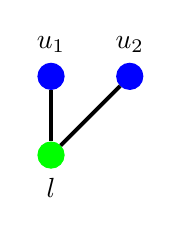
\begin{tikzpicture}
		\node[shape=circle,draw=blue,fill=blue,label=above:$u_1$] (u1) {};
		\node[shape=circle,draw=blue,fill=blue,label=above:$u_2$] (u2) [right of=u1] {};
		\node[shape=circle,draw=green,fill=green,label=below:$l$] (l) [midway, below of=u1] {};

		\draw (u1) [line width=0.5mm] -- (l);
		\draw (u2) [line width=0.5mm] -- (l);
		\end{tikzpicture}
	\caption{Wedge}
	\label{fig:wedge-example}
\end{subfigure}
\begin{subfigure}[b]{0.3\textwidth}
	\centering
 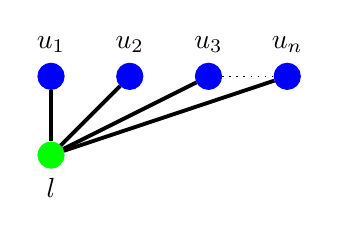
\begin{tikzpicture}
	\node[shape=circle,draw=blue,fill=blue,label=above:$u_1$] (u1) {};
	\node[shape=circle,draw=blue,fill=blue,label=above:$u_2$] (u2) [right of=u1] {};
	\node[shape=circle,draw=blue,fill=blue,label=above:$u_3$] (u3) [right of=u2] {};
	\node[shape=circle,draw=blue,fill=blue,label=above:$u_n$] (un) [right of=u3] {};
	\node[shape=circle,draw=green,fill=green,label=below:$l$] (l) [midway, below of=u2] {};

	\draw (u1) [line width=0.5mm] -- (l);
	\draw (u2) [line width=0.5mm] -- (l);
	\draw (u3) [line width=0.5mm] -- (l);
	\draw (un) [line width=0.5mm] -- (l);
	\draw (u3) [dotted,line width=0.2mm] -- (un);
	\end{tikzpicture}
\caption{Aggregated Wedge}
\label{fig:agg-wedge-example}
\end{subfigure}
\begin{subfigure}[b]{0.3\textwidth}
	\centering
 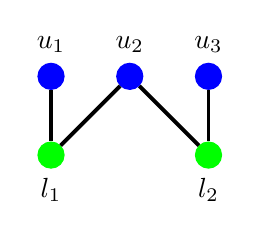
\begin{tikzpicture}
	\node[shape=circle,draw=blue,fill=blue,label=above:$u_1$] (u1) {};
	\node[shape=circle,draw=blue,fill=blue,label=above:$u_2$] (u2) [right of=u1] {};
	\node[shape=circle,draw=blue,fill=blue,label=above:$u_3$] (u3) [right of=u2] {};
	\node[shape=circle,draw=green,fill=green,label=below:$l_1$] (l1) [below of=u1] {};
	\node[shape=circle,draw=green,fill=green,label=below:$l_2$] (l2) [below of=u3] {};

	\draw (u1) [line width=0.5mm] -- (l1);
	\draw (u2) [line width=0.5mm] -- (l1);
	\draw (u2) [line width=0.5mm] -- (l2);
	\draw (u3) [line width=0.5mm] -- (l2);
\end{tikzpicture}
\caption{Double Wedge}
\label{fig:double-wedge-example}
\end{subfigure}
\end{figure}

 